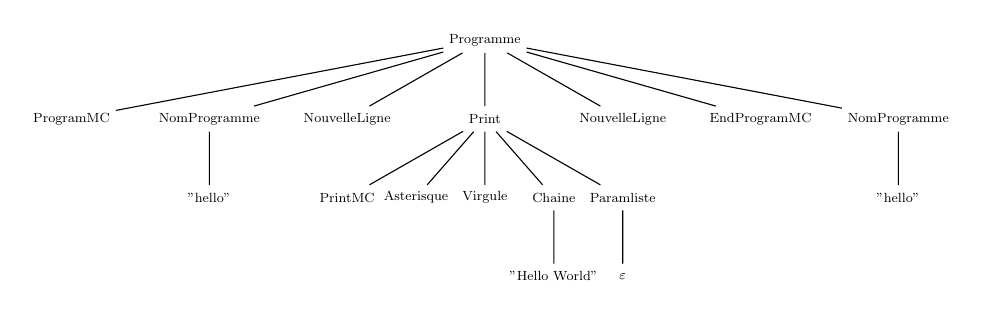
\begin{tikzpicture}
    [
        baseline=(base),
        level/.style={sibling distance = 1.75cm/#1, level distance = 1cm},
        every node/.style={scale=0.6, font=\footnotesize, minimum width=15pt, minimum height=15pt}
    ]
    
    \node {Programme}
        child {node (base) {ProgramMC}}
        child {node {NomProgramme}
            child {node {"hello"}}
        }
        child {node {NouvelleLigne}}
        child {node {Print}
            child {node {PrintMC}}
            child {node {Asterisque}}
            child {node {Virgule}}
            child {node {Chaine}
                child {node {"Hello World"}}
            }
            child{node {Paramliste}
                child {node {$\varepsilon$}}
            }
        }
        child {node {NouvelleLigne}}
        child {node {EndProgramMC}}
        child {node {NomProgramme}
            child {node {"hello"}}
        }
    ;
\end{tikzpicture}